\section{Theoretical Models of Rapport for Agents}
\label{sec:ComputationalModelsOfRapport}

Rapport is a mostly unconscious phenomenon~\cite{Zwiers2011} that occurs during interactions marked by strong perceptions of coordination, positivity and mutual attention.

The most important concepts for managing rapport are: planning social behaviours (Figure~\ref{table:BuildingRapportPlan}), learning social behaviours and flexible mechanisms to regulate current actions. Rapport models involve several complex cognitive processes. Therefore it is useful to discretise it into smaller sets capable of, for example, enhancing positivity (friendliness) using self-disclosure or enhancing coordination and attentiveness through backchannel and turn-taking strategies~\cite{Sacks1974, Kahn2008, Welbergen2012}. The latter strategies are allied with good listeners as they must able to understand how to provide well-timed adequate feedback (backchannel) and identify appropriate moments to become the speaker (turn-taking) and encourage further dialogue~\cite{Sacks1974, Poppe2010}.

Zhao, Papangelis, and Cassell, propose a theoretical model to manage long-term rapport~\cite{Zhao2014, Papangelis2014} that is very relevant for current implementations of long-term social companionship agents~\cite{Lisetti2013, Bickmore2005, Kang2005}. Similarly to what was described previously in Chapter~\ref{chap:rapport}, the proposed model treats rapport as an interactional goal (Figure~\ref{table:BuildingRapportPlan}) that is satisfied through strategies tailored to the user and the state of the interaction (Table~\ref{table:TCArchitectureDyadicRapportManagement:State}). These strategies, despite initially representing the general sociocultural norms, must adapt to the interpersonal norms of the relationship and the context~\cite{Zhao2014}. As the relationship evolves, the dyadic state and the internal models should be updated in order to store the most accurate description of the interaction and return finer behavioural responses that satisfy the dyad behavioural expectations~\cite{Papangelis2014}.


\begin{table}[H]
	\centering
	\begin{tabular}{|l|l|}
	\hline
	\textbf{Dyadic State} & Rapport state; Behavioural model; Friendship status; History \\ \hline
	\textbf{User Model} & User goals; Shared knowledge; Task model; User's putative dyadic State \\ \hline
	\end{tabular}
    \caption{Required data structures to manage rapport as proposed by Zhao et. al.~\cite{Zhao2014}.}
    \label{table:TCArchitectureDyadicRapportManagement:State}
\end{table}

Another important aspect of rapport management is the ability to continuously adapt to the current interaction and environment, give incremental feedback~\cite{Kopp2007, Zwiers2011, Reidsma2011, Visser2014}, and even recover from mistakes~\cite{Kahn2008}. Its usefulness is remarked on complex synchronised behaviours such as speech and handshakes~\cite{Zwiers2011}. This requires incremental planning and execution of behavioural chunks that can be potentially interrupted, modified, and even replaced~\cite{Reidsma2011, Visser2014, Kopp2007, Zwiers2011}. 

Most \ac{HRI} agents follow the SAIBA model~\cite{Niewiadomski2009,Buschmeier2011,Hartholt2013,Tullio2015} (Figure~\ref{fig:saiba}) that consists of a pipeline of three decoupled components: the intentions planner responsible for generating the desired intentions using \ac{FML}; the behaviour planning responsible for translating intentions (\ac{FML}) into behaviours (e.g., where to look and what to say) using \ac{BML}; lastly, the realisation planner responsible for executing the \ac{BML} on the agent (virtual or robotic)~\cite{Kopp2006}. In order to handle interruptions, modifications or even replacement of ongoing actions, researchers suggest that the current \ac{BML} specification should be extended to better support synchronisation, anticipation and prediction of behaviours between the members of an interaction~\cite{Kopp2006, Kopp2007, Zwiers2011, Reidsma2011}. For example, by adding information the BML on how behaviours should be elegantly interrupted (i.e., in a natural and socially adequate manner) depending on the current state of the interaction~\cite{Zwiers2011}.

\begin{figure}[H]
	\centering
	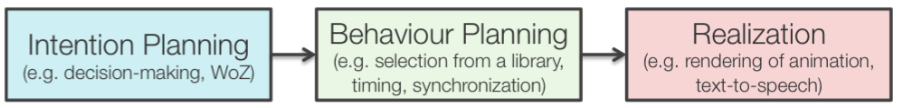
\includegraphics[width=0.85\textwidth]{images/SAIBA.png}
	\caption{The SAIBA model for virtual agents. From~\cite{Tullio2015}.}
	\label{fig:saiba}
\end{figure}


